\needspace{10\baselineskip}
\SourceLeaf{325}
\pdfbookmark[1]{18. Zodiak[u]s}{zusatz-018}
\begin{center}
[18.]

Zodiak[u]s.
\end{center}

[Um ein Beispiel für den Fall zu erhalten, wo zwei Limiten die Himmelskugel in mehrere Stücke scheiden, und wo einige dieser Stücke gar keine geocentrische Örter enthalten, andere solche, die auf zwei Arten, wieder andere solche, die auf vier Arten geocentrische Örter sein können, wähle man für die]
\[
\begin{aligned}
\text{Äussere Bahn}\quad &k=1&\qquad e&=0\\
\text{Innere Bahn}\quad &k^{\prime}=0{,}8&g^{\prime}&=270^{0}
\end{aligned}
\qquad [i=90^{0}]
\]
[wo die Bezeichnungen dieselben sind, wie in der Abhandlung »Über die Grenzen der geocentrischen Örter etc.« Band VI S. 106. Man hat dann die]
\[
\begin{aligned}
\text{Formeln:}\qquad &\cos t^{\prime}=\frac{k^{\prime}}{k}\cos t\\[5pt]
&r^{\prime}=\frac{k^{\prime}}{1-e^{\prime}\sin t^{\prime}}\\[5pt]
&r^{\prime}\cos t^{\prime}-k\cos t=\Delta\cos\alpha\cos\beta\\[5pt]
&-k\sin t=\Delta\sin\alpha\cos\beta\\[5pt]
&r^{\prime}\sin t^{\prime}=\Delta\sin\beta.
\end{aligned}
\]

[In diesem Falle existiren zwei getrennte Limitenlinien, welche sich selbst schneiden können, und zwar findet sich die] critische Stelle [für]
\[
\sin t^{\prime}=\BareRoot[3]{\frac{1-\dfrac{k^{\prime}k^{\prime}}{kk}}{e^{\prime}}}\mathpunct{\cdot}
\]
[Es sind hier vier Typen von Limiten zu unterscheiden, für welche die folgenden Zahlen Beispiele geben:]
\begin{center}
Bahn I.\\[3pt]
Critische Stelle \(t=90^{0}\)\\
\(e^{\prime}=0{,}36\)\\
\(\log e^{\prime}=9{,}55630\)\par\smallskip
\begin{tabular}{r@{\qquad}r@{\qquad}r}
\(t\)&\([\alpha]\)&\([\beta]\)\\[3pt]
\(0^{0}\)&\(180^{0}\quad0^{\prime}\)&\(73^{0}\,18^{\prime}\)\\
\(15\)&\(237\quad32\)&\(65\quad1\)\\
\(30\)&\(256\quad47\)&\(56\quad36\)\\
\(45\)&\(264\quad52\)&\(52\quad53\)\\
\(60\)&\(268\quad31\)&\(51\quad38\)\\
\(75\)&\(269\quad49\)&\(51\quad22\)\\
\(90\)&\(270\quad0\)&\(51\quad20\)
\end{tabular}
\end{center}
\SourceLeaf{326}
\begin{center}
Bahn II.\\[3pt]
Critische Stelle \(t=75^{0}\)\\
\(e^{\prime}=0{,}38446\)\\
\(\log e^{\prime}=9{,}58485\)\par\smallskip
\begin{tabular}{r@{\qquad}r@{\qquad}r}
\(t\)&\([\alpha]\)&\([\beta]\)\\[3pt]
\(0^{0}\)&\(180^{0}\quad0^{\prime}\)&\(74^{0}\,55^{\prime}\)\\
\(15\)&\(240\quad12\)&\(66\quad3\)\\
\(30\)&\(258\quad47\)&\(57\quad26\)\\
\(45\)&\(266\quad24\)&\(53\quad44\)\\
\(60\)&\(269\quad37\)&\(52\quad35\)\\
\(63^{0}\,59^{\prime}\)&\(270\quad0\)&\(52\quad29\)\\
\(75\)&\(270\quad25\)&\(52\quad24\)\\
\(90\)&\(270\quad0\)&\(52\quad26\)
\end{tabular}
\end{center}
\begin{center}
Bahn III.\\[3pt]
[Critische Stelle] \(t=60^{0}\)\\
\(e^{\prime}=0{,}46761\)\\
\(\log e^{\prime}=9{,}66988\)\par\smallskip
\begin{tabular}{r@{\qquad}r@{\qquad}r}
\(t\)&\([\alpha]\)&\([\beta]\)\\[3pt]
\(0^{0}\)&\(180^{0}\quad0^{\prime}\)&\(80^{0}\,36^{\prime}\)\\
\(15\)&\(251\quad27\)&\(69\quad17\)\\
\(30\)&\(266\quad35\)&\(60\quad5\)\\
\(37^{0}\quad5^{\prime}\)&\(270\quad0\)&\(57\quad56\)\\
\(45\)&\(272\quad23\)&\(56\quad37\)\\
\(60\)&\(273\quad58\)&\(55\quad55\)\\
\(75\)&\(272\quad45\)&\(56\quad10\)\\
\(90\)&\(270\quad0\)&\(56\quad21\)
\end{tabular}
\end{center}
\begin{center}
Bahn IV.\\[3pt]
\(e^{\prime}=0{,}6\)\\
\(\log e^{\prime}=9{,}77815\)\\
Critische Stelle \(t=47^{0}\,48^{\prime}\,49^{\prime\prime}\)\par\smallskip
\begin{tabular}{r@{\qquad}r@{\qquad}r}
\(t\)&\([\alpha]\)&\([\beta]\)\\[3pt]
\(0^{0}\)&\(270^{0}\quad0^{\prime}\)&\(90^{0}\quad0^{\prime}\)\\
\(15\)&\(277\quad10\)&\(72\quad21\)\\
\(30\)&\(282\quad31\)&\(63\quad16\)\\
\(45\)&\(284\quad56\)&\(60\quad44\)\\
\(47^{0}\,49^{\prime}\)&\(285\quad0\)&\(60\quad41\)\\
\(60\)&\(283\quad41\)&\(61\quad19\)\\
\(75\)&\(278\quad23\)&\(62\quad45\)\\
\(90\)&\(270\quad0\)&\(63\quad26.\)
\end{tabular}
\end{center}

[Die Rechnung ist nur für die nördliche Limitenlinie ausgeführt und für diese lässt sich] also bei symmetrischer Lage der Übergang [von einem Typus zum andern durch die folgenden Figuren darstellen:]
\SourceLeaf{327}
\begin{center}
\begin{tabular}{@{}ccc@{}}
\begin{tikzpicture}[x=.5pt,y=-.5pt,line width=.65pt,line cap=round,line join=round,font=\scriptsize]
\useasboundingbox (125,240) rectangle (335,590);
\draw (269,253) .. controls (289,250) and (298,276) .. (301,315)
 .. controls (309,388) and (306,464) .. (276,470)
 .. controls (244,480) and (237,422) .. (236,366)
 .. controls (233,313) and (238,252) .. (269,253);
\fill (270,361) circle[radius=1.1pt];
\node at (270,349) {0};\node at (222,349) {2};\node at (315,349) {2};
\node at (180,518) {[Bahn]};\node at (270,518) {I};
\node at (270,570) {\(\mathrm{E}\leqq0.36\)};
\end{tikzpicture}
&
\begin{tikzpicture}[x=.5pt,y=-.5pt,line width=.65pt,line cap=round,line join=round,font=\scriptsize]
\useasboundingbox (390,240) rectangle (580,590);
\draw (466,253) .. controls (481,255) and (498,255) .. (510,253);
\draw (466,253) .. controls (504,283) and (520,326) .. (519,364)
 .. controls (518,411) and (491,449) .. (464,470);
\draw (510,253) .. controls (475,281) and (457,324) .. (457,362)
 .. controls (455,408) and (481,447) .. (508,470);
\draw (464,470) .. controls (480,468) and (494,468) .. (508,470);
\fill (488,359) circle[radius=1.1pt];
\node at (488,348) {0};\node at (534,348) {2};\node at (488,263) {4};
\node at (488,518) {II};
\end{tikzpicture}
&
\begin{tikzpicture}[x=.5pt,y=-.5pt,line width=.65pt,line cap=round,line join=round,font=\scriptsize]
\useasboundingbox (610,240) rectangle (800,590);
\draw (657,255) .. controls (688,265) and (722,267) .. (750,257);
\draw (657,255) .. controls (689,283) and (712,325) .. (713,363)
 .. controls (715,406) and (692,445) .. (660,472);
\draw (750,257) .. controls (719,283) and (696,324) .. (696,363)
 .. controls (694,409) and (720,452) .. (752,476);
\draw (660,472) .. controls (692,464) and (725,464) .. (752,476);
\fill (704,366) circle[radius=1.1pt];
\node at (704,353) {0};\node at (727,353) {2};\node at (704,284) {4};
\node at (704,520) {III};
\end{tikzpicture}
\\[9pt]
\begin{tikzpicture}[x=.5pt,y=-.5pt,line width=.65pt,line cap=round,line join=round,font=\scriptsize]
\useasboundingbox (830,240) rectangle (1020,590);
\draw (870,263) .. controls (902,275) and (946,278) .. (975,265);
\draw (870,263) .. controls (901,289) and (922,329) .. (923,352)
 -- (923,382) .. controls (921,423) and (898,458) .. (871,478);
\draw (975,265) .. controls (945,290) and (925,330) .. (923,352)
 -- (923,382) .. controls (925,424) and (949,460) .. (979,480);
\draw (871,478) .. controls (906,465) and (946,468) .. (979,480);
\node at (923,299) {4};\node at (947,357) {2};
\node at (923,526) {IV};\node at (928,575) {\(\mathrm{E}=0.6\)};
\end{tikzpicture}
&
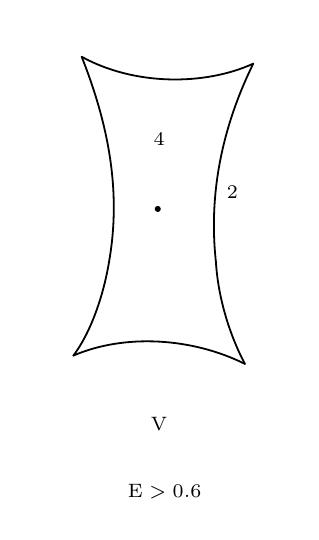
\begin{tikzpicture}[x=.5pt,y=-.5pt,line width=.65pt,line cap=round,line join=round,font=\scriptsize]
\useasboundingbox (1040,240) rectangle (1230,590);
\draw (1079,261) .. controls (1117,282) and (1168,282) .. (1203,266);
\draw (1079,261) .. controls (1100,314) and (1107,361) .. (1099,408)
 .. controls (1094,439) and (1083,464) .. (1073,477);
\draw (1203,266) .. controls (1179,315) and (1171,363) .. (1176,409)
 .. controls (1178,442) and (1190,470) .. (1197,483);
\draw (1073,477) .. controls (1110,461) and (1159,464) .. (1197,483);
\fill (1134,371) circle[radius=1.1pt];
\node at (1135,321) {4};\node at (1188,359) {2};
\node at (1135,526) {V};\node at (1139,575) {\(\mathrm{E}>0.6\)};
\end{tikzpicture}
&
\end{tabular}
\end{center}

[Als Mittelpunkt der Figuren ist der Nordpol der innern Bahn vorzustellen; die Zahlen in den Figuren bedeuten die Anzahl der Arten, auf welche die betreffenden Theile der Himmelskugel geocentrische Örter sein können.]
\begin{center}\rule{.22\textwidth}{.3pt}\end{center}
